\documentclass{article}
\usepackage{hyperref}
\usepackage{listings}
\usepackage{color}
\usepackage{graphicx}
\title{GitHub Activity Tracker}
\author{Emanuele Nuzzo}
\date{\today}

\begin{document}

\maketitle

\section{Objective}
The objective of this assignment is to track activities on GitHub using the GitHub Events API. The application monitors up to five configurable repositories and generates statistics based on a rolling window of either 7 days or 500 events, whichever is less. These statistics are made available to end-users via a REST API, showing the average time between consecutive events for each combination of event type and repository name.

\section{Features}
\begin{itemize}
    \item Monitors up to five configurable repositories.
    \item Generates statistics based on a rolling window of 7 days or 500 events.
    \item Provides a REST API to access the statistics.
    \item Minimizes requests to the GitHub API.
    \item Retains data through application restarts.
\end{itemize}

\section{Assumptions}
\begin{itemize}
    \item The GitHub Events API is used to fetch events.
    \item The application is designed to handle up to five repositories.
    \item The rolling window is either 7 days or 500 events, whichever is less.
    \item The application is implemented in Python.
\end{itemize}

\section{Installation and Setup}
\begin{enumerate}
    \item \textbf{Clone the repository:}
    \begin{lstlisting}[language=bash]
    git clone https://github.com/emanuzzo/github_activity_tracker.git
    cd github_activity_tracker
    \end{lstlisting}
    
    \item \textbf{Create a virtual environment and activate it:}
    \begin{lstlisting}[language=bash]
    python -m venv venv
    source venv/bin/activate  # On Windows use `venv\Scripts\activate`
    \end{lstlisting}
    
    \item \textbf{Install the required dependencies:}
    \begin{lstlisting}[language=bash]
    pip install -r requirements.txt
    \end{lstlisting}
    
    \item \textbf{Configure the repositories to be tracked:}
    Edit the \texttt{config.json} file to include the repositories you want to monitor.
    
    \item \textbf{Run the application:}
    \begin{lstlisting}[language=bash]
    python app.py
    \end{lstlisting}
\end{enumerate}

\section{Usage}
\begin{itemize}
    \item \textbf{API Endpoint:} \url{http://127.0.0.1:5000/stats}
    \item \textbf{Response Format:}
    \begin{lstlisting}[language=json]
    {
      "repository_name": {
        "event_type": "average_time_between_events"
      }
    }
    \end{lstlisting}
\end{itemize}



\section{Code Overview}
\begin{itemize}
    \item \textbf{app.py:} main application file that sets up the Flask server and handles API requests.
    \item \textbf{config.py:} configuration file that allow to consume, with the generated token, the 5 repository api. 
    \item \textbf{github\_events.db:} SQL lite db created from the application at the first run.
\end{itemize}

\section{Example Response}
This is an example of the stats we can get from this application
\clearpage

\begin{figure}
    \centering
    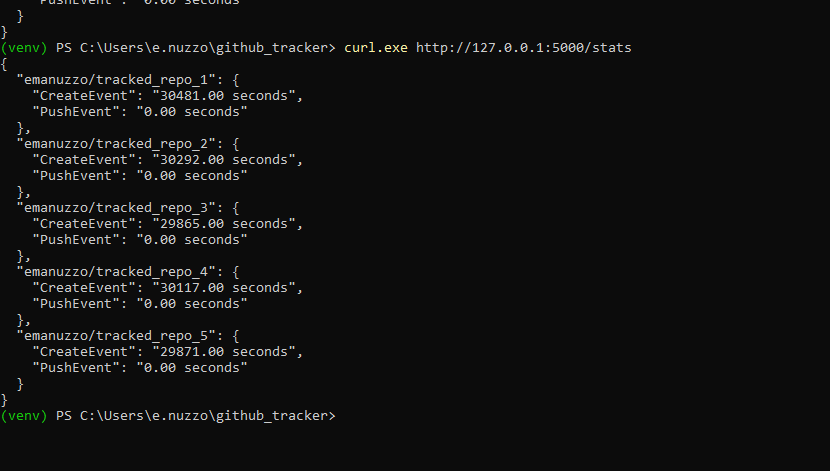
\includegraphics[width=0.5\linewidth]{image.png}
\end{figure}

\section{API Documentation}
\subsection{GET /stats}
\begin{itemize}
    \item \textbf{Description:} Retrieves the average time between consecutive events for each combination of event type and repository name.
    \item \textbf{Response:} JSON object containing the statistics.
\end{itemize}

\section{Conclusion}
This application provides a robust solution for tracking GitHub activities across multiple repositories, offering valuable insights through a simple REST API.

\end{document}
